\documentclass[14pt,a4paper,report]{report}
\usepackage[a4paper, mag=1000, left=2.5cm, right=1cm, top=2cm, bottom=2cm, headsep=0.7cm, footskip=1cm]{geometry}
\usepackage[utf8]{inputenc}
\usepackage[english,russian]{babel}
\usepackage{indentfirst}
\usepackage[dvipsnames]{xcolor}
\usepackage[colorlinks]{hyperref}
\usepackage{listings} 
\usepackage{fancyhdr}
\usepackage{caption}
\usepackage{graphicx}
\hypersetup{
	colorlinks = true,
	linkcolor  = black
}

\usepackage{titlesec}
\titleformat{\chapter}
{\Large\bfseries} % format
{}                % label
{0pt}             % sep
{\huge}           % before-code


\DeclareCaptionFont{white}{\color{white}} 

% Listing description
\usepackage{listings} 
\DeclareCaptionFormat{listing}{\colorbox{gray}{\parbox{\textwidth}{#1#2#3}}}
\captionsetup[lstlisting]{format=listing,labelfont=white,textfont=white}
\lstset{ 
	% Listing settings
	inputencoding = utf8,			
	extendedchars = \true, 
	keepspaces = true, 			  	 % Поддержка кириллицы и пробелов в комментариях
	language = bash,            	 	 % Язык программирования (для подсветки)
	basicstyle = \small\sffamily, 	 % Размер и начертание шрифта для подсветки кода
	numbers = left,               	 % Где поставить нумерацию строк (слева\справа)
	numberstyle = \tiny,          	 % Размер шрифта для номеров строк
	stepnumber = 1,               	 % Размер шага между двумя номерами строк
	numbersep = 5pt,              	 % Как далеко отстоят номера строк от подсвечиваемого кода
	backgroundcolor = \color{white}, % Цвет фона подсветки - используем \usepackage{color}
	showspaces = false,           	 % Показывать или нет пробелы специальными отступами
	showstringspaces = false,    	 % Показывать или нет пробелы в строках
	showtabs = false,           	 % Показывать или нет табуляцию в строках
	frame = single,              	 % Рисовать рамку вокруг кода
	tabsize = 2,                  	 % Размер табуляции по умолчанию равен 2 пробелам
	captionpos = t,             	 % Позиция заголовка вверху [t] или внизу [b] 
	breaklines = true,           	 % Автоматически переносить строки (да\нет)
	breakatwhitespace = false,   	 % Переносить строки только если есть пробел
	escapeinside = {\%*}{*)}      	 % Если нужно добавить комментарии в коде
}

\begin{document}

\def\contentsname{Содержание}

% Titlepage
\begin{titlepage}
	\begin{center}
		\textsc{Санкт-Петербургский Политехнический 
			Университет Петра Великого\\[5mm]
			Кафедра компьютерных систем и программных технологий}
		
		\vfill
		
		\textbf{Отчёт по лабораторной работе №3\\[3mm]
			Курс: «Защита информации»\\[6mm]
			Тема: «Ознакомление с PGP системами на основе программы Kleopatra»\\[35mm]
		}
	\end{center}
	
	\hfill
	\begin{minipage}{.5\textwidth}
		Выполнил студент:\\[2mm] 
		Бояркин Никита Сергеевич\\
		Группа: 43501/3\\[5mm]
		
		Проверил:\\[2mm] 
		Новопашенный Андрей Гелиевич
	\end{minipage}
	\vfill
	\begin{center}
		Санкт-Петербург\\ \the\year\ г.
	\end{center}
\end{titlepage}

% Contents
\tableofcontents
\clearpage

\chapter{Лабораторная работа №3}

\section{Цель работы}

Ознакомиться с PGP системами на основе программы Kleopatra.

\section{Программа работы}

\begin{enumerate}
	\item Ознакомиться с программой Kleopatra.
	\item Создать новый сертификат.
	\item Зашифровать произвольный файл открытым ключем.
	\item Расшифровать произвольный файл закрытым ключем.
\end{enumerate}

\section{Программное окружение}

\subsubsection{Первый компьютер}

\lstinputlisting{listings/1.0.log}

\subsubsection{Второй компьютер}

\lstinputlisting{listings/2.0.log}

\section{Ход работы}

\subsection{Pretty Good Privacy}

Pretty Good Privacy (PGP) — компьютерная программа, также библиотека функций, позволяющая выполнять операции шифрования и цифровой подписи сообщений, файлов и другой информации, представленной в электронном виде, в том числе прозрачное шифрование данных на запоминающих устройствах, например, на жёстком диске. Первоначально разработана Филиппом Циммерманном в 1991 году.

В 1999 году силами Фонда свободного программного обеспечения была создана свободная реализация OpenPGP под названием GNU Privacy Guard (GnuPG).

В рамках данной лабораторной работы ограничимся изучением менеджера сертификатов Kleopatra, который включается в OpenPGP реализацию.

\subsection{Принцип работы}

Первым этапом является создание нового сертификата. Генерируется пара ключей: открытый ключ и закрытый ключ. Ключи являются парными, и файлы зашифрованные одним ключем можно расшифровать только парным ключем. Открытый ключ распространяется открыто, в то время как закрытый ключ должен сохраняться в секрете. Стоит отметить, что в программе Kleopatra доступ к расшифровке закрытым ключем защищается специальным паролем.

Таким образом, сторона создающая сертификат распространяет открытый ключ среди пользователей, от которых ожидается прием сообщений. Сообщения шифруются этим открытым ключем на стороне пользователя и пересылаются стороне, создавшей сертификат. После этого, сторона создавшая сертификат расшифровывает сообщение закрытым ключем.

\subsection{Создание сертификата}

Проиллюстрируем этап создания нового сертификата (File -> New Certificate...). Первый этап - выбор стандарта для пары ключей. Kleopatra поддерживает помимо OpenPGP также и X.509: 

\begin{figure}[h!]
	\centering
	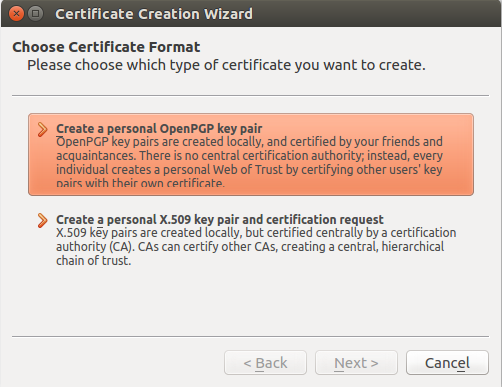
\includegraphics[scale = 0.68]{images/1_1.png}
	
	\caption{Выбор стандарта для пары ключей}
	\label{image:1}
\end{figure}

После этого происходит процесс конфигурирования сертификата (выбор алгоритма шифрования, длины ключа, названия сертификата и др.):

\begin{figure}[h!]
	\centering
	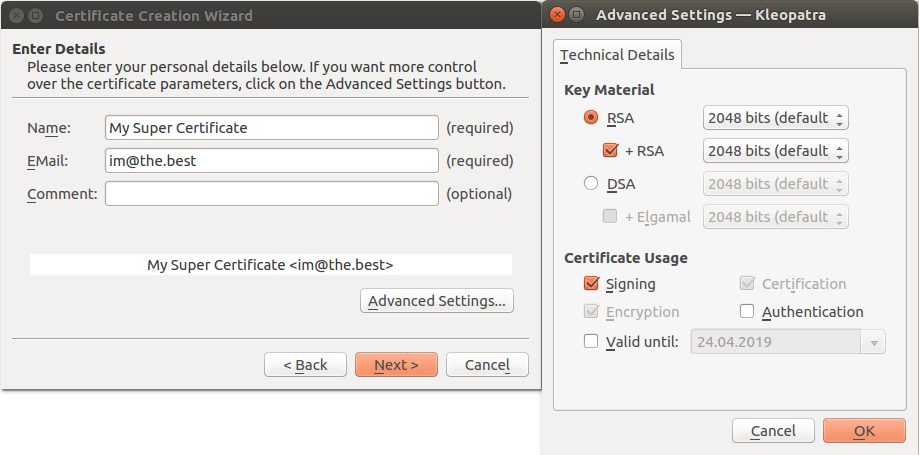
\includegraphics[scale = 0.68]{images/1_2.png}
	
	\caption{Конфигурирование сертификата и выбор алгоритма шифрования}
	\label{image:2}
\end{figure}

Затем, происходит процесс генерирования пары ключей (на основе случайных символов и движения окна), а также устанавливается пароль на доступ к закрытому ключу:

\begin{figure}[h!]
	\centering
	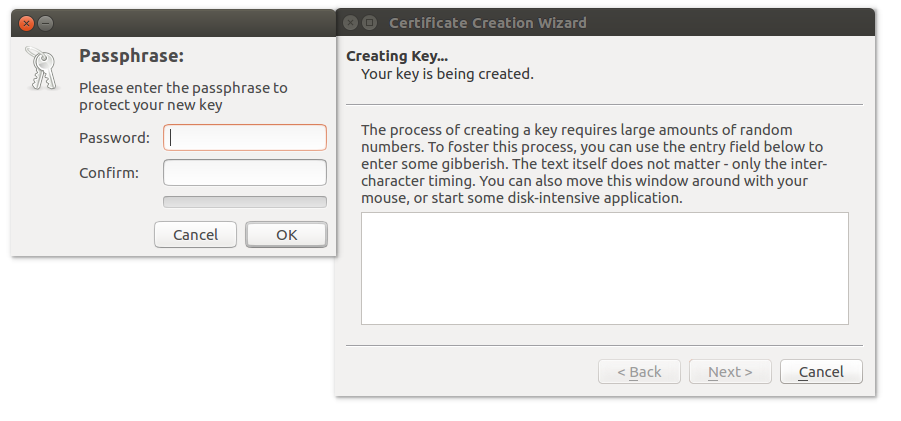
\includegraphics[scale = 0.65]{images/1_3.png}
	
	\caption{Процесс генерирования пары ключей и установление пароля на доступ к закрытому ключу}
	\label{image:3}
\end{figure}

Созданный сертификат появляется в списке сертификатов:

\begin{figure}[h!]
	\centering
	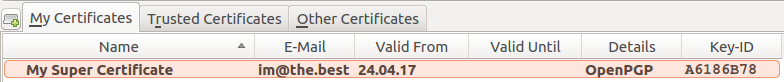
\includegraphics[scale = 0.65]{images/1_4.png}
	
	\caption{Результат создания сертификата}
	\label{image:4}
\end{figure}

Для получения открытого ключа воспользуемся командой ПКМ -> Export Certificates... Отрытый ключ сохраняется в файле с собственным расширением:

\begin{figure}[h!]
	\centering
	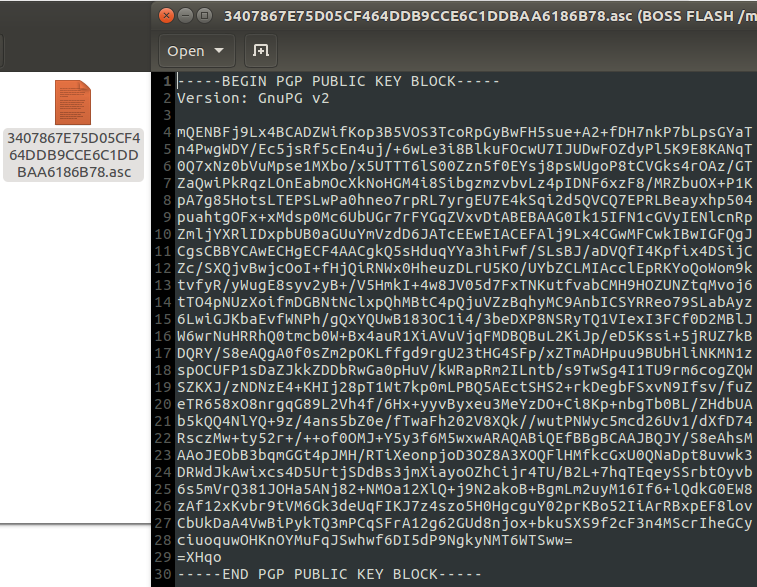
\includegraphics[scale = 0.65]{images/1_5.png}
	
	\caption{Открытый ключ RSA 2048 бит}
	\label{image:5}
\end{figure}

Этот файл можно распространять среди пользователей, от которых ожидается прием сообщений.

\clearpage

\subsection{Шифрование файлов открытым ключем}

На втором компьютере импортируем сертификат (File -> Import Certificates...), указав в качестве параметра созданный открытый ключ (см. п. 1.4.3):

\begin{figure}[h!]
	\centering
	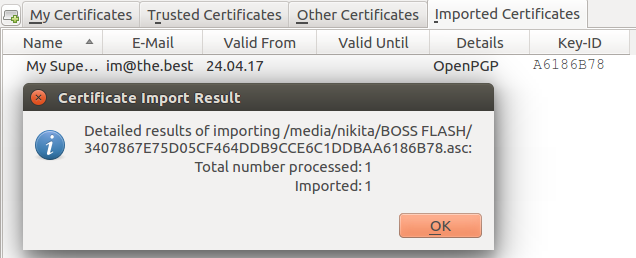
\includegraphics[scale = 0.55]{images/2_1.png}
	
	\caption{Результат импортирования сертификата}
	\label{image:6}
\end{figure}

Для шифрования файлов воспользуемся командой File -> Sign/Encrypt files... Появляется окно с выбором параметров шифрования:

\begin{figure}[h!]
	\centering
	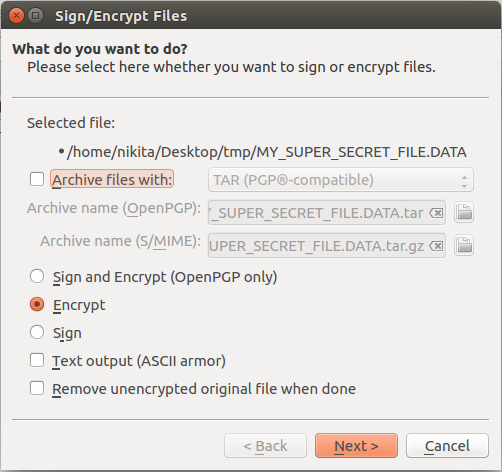
\includegraphics[scale = 0.53]{images/2_2.png}
	
	\caption{Выбор параметров шифрования}
	\label{image:7}
\end{figure}

Далее указывается сертификат для шифрования файла:

\begin{figure}[h!]
	\centering
	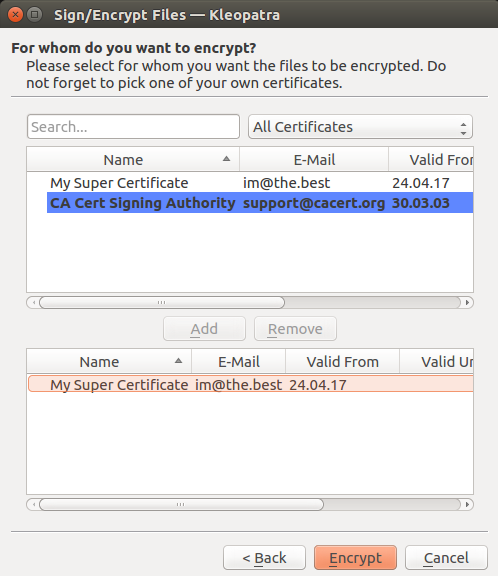
\includegraphics[scale = 0.53]{images/2_3.png}
	
	\caption{Выбор сертификата для шифрования}
	\label{image:8}
\end{figure}

Результат шифрования файла:

\begin{figure}[h!]
	\centering
	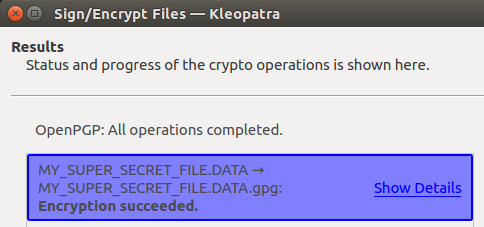
\includegraphics[scale = 0.53]{images/2_4.png}
	
	\caption{Результат шифрования файла}
	\label{image:9}
\end{figure}

Файл был зашифрован в формате .gpg, расшифровка этого файла возможна только закрытым ключем, поэтому расшифровать его на этом компьютере нельзя, даже учитывая что мы его и зашифровали.

\subsection{Расшифровка файлов закрытым ключем}

Для расшифровки файлов воспользуемся командой File -> Decrypt/Verify files... Появляется окно с выбором параметров расшифровки:

\begin{figure}[h!]
	\centering
	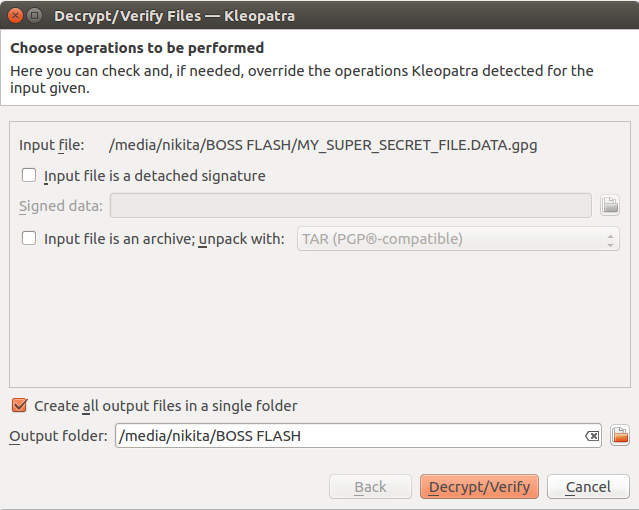
\includegraphics[scale = 0.51]{images/1_6.png}
	
	\caption{Выбор параметров расшифровки}
	\label{image:10}
\end{figure}

Для доступа к расшифровке закрытым ключем необходимо ввести пароль, который был создан вместе с сертификатом (см. п. 1.4.3):

\begin{figure}[h!]
	\centering
	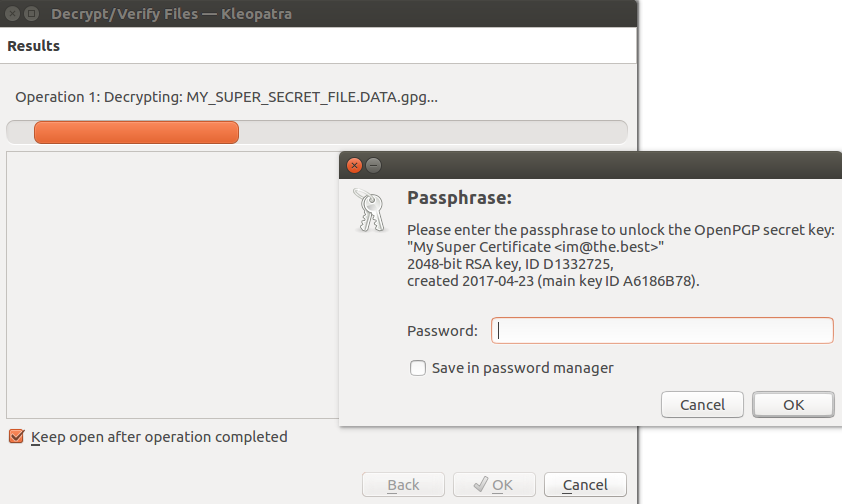
\includegraphics[scale = 0.51]{images/1_7.png}
	
	\caption{Расшифровка закрытым ключем}
	\label{image:11}
\end{figure}

Результат расшифровки файла:

\begin{figure}[h!]
	\centering
	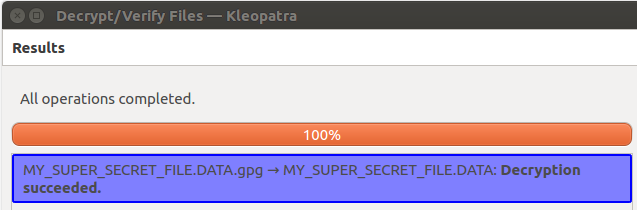
\includegraphics[scale = 0.63]{images/1_8.png}
	
	\caption{Результат расшифровки файла}
	\label{image:12}
\end{figure}

Файл был успешно расшифрован: название и содержимое файла совпадает с оригиналом.

\section{Вывод}

В данной работе было рассмотрено ассиметричное шифрование на примере программы Kleopatra семейства OpenPGP. Ассиметричное шифрование имеет преимущество перед симметричным в простоте обмена ключами, однако проигрывает в скорости шифрования. Рассмотренное в работе шифрование одностороннее. Для того, чтобы осуществить двустороннюю передачу используются два канала. В современных криптосистемах ассиметричное шифрование используется для обмена ключами, а одновременно с этим симметричное шифрование для обмена данными.

\end{document}